\documentclass[unicode]{beamer}
\usepackage{cmap}
\usepackage[T2A]{fontenc}
\usepackage[utf8]{inputenc}
\usepackage[english, russian]{babel}
\usepackage{amsmath,mathrsfs,amsfonts,amssymb}
\usepackage{graphicx, epsfig}
\usepackage{subfig}
\usepackage[noend]{algorithmic}

\usepackage{graphicx, epsfig}
\graphicspath{{pictures/}}
\DeclareGraphicsExtensions{.pdf,.png,.jpg}
\usepackage{subfig}
\usepackage{color}
\usepackage{gensymb}



\usepackage{algpseudocode}
\renewcommand{\algorithmicend}{\textbf{завершим}}
\renewcommand{\algorithmicif}{\textbf{если}}
\renewcommand{\algorithmicelse}{\textbf{иначе}}
\renewcommand{\algorithmicthen}{\textbf{то}}



\usetheme{Warsaw}%{Singapore}%{Warsaw}%{Warsaw}%{Darmstadt}
\usecolortheme{sidebartab}
\setbeamertemplate{footline}[author, institute]
\expandafter\def\expandafter\insertshorttitle\expandafter{%
  \insertshorttitle\hfill%
  \insertframenumber\,/\,\inserttotalframenumber}

% отключить клавиши навигации
\setbeamertemplate{navigation symbols}{}


\title[]{Модификация почвенно-снежного блока климатической модели ИВМ РАН}
\author[CITES2021: Разработка компонент модели системы Земля]{Черненков Алексей Юрьевич$^{1, *}$, Кострыкин Сергей Владимирович$^{2-4, **}$, Володин Евгений Михайлович$^{2, ***}$}
\institute[]{
    $^1$Московский физико-технический институт (национальный исследовательский университет)
    
    $^2$Институт вычислительной математики им. Г.И. Марчука РАН
    
    $^3$Институт глобального климата и экологии им. Ю.А. Израэля
    
    $^4$Институт физики атмосферы им. А.М.Обухова РАН
}

\date{
    \footnotesize
    26 ноября 2021 г.
}

\begin{document}

% Creates title page of slide show using above information
\begin{frame}
  \titlepage
\end{frame}



\begin{frame}{- - вводные слова, разнае типы снега, таяние, перезамерзание... предпосылки к появлению данной работы (необходимость переменных для модели альбедо) - -}
    
\end{frame}



\begin{frame}{Климатическая модель ИВМ РАН}

\begin{itemize}
    \item Рассматривается пятая версия INMCM5\footnote{\tiny Volodin, Evgeny and Mortikov, Evgeny and Kostrykin, Sergey and Galin, V. and Lykossov, Vasily and Gritsun, Andrey and Diansky, Nikolay and Gusev, Anatoly and Iakovlev, Nikolay. Simulation of the present-day climate with the climate model INMCM5. Climate Dynamics, 2017, Vol. 49, DOI: 10.1007/s00382-017-3539-7.} 
    \item Она представляет собой модель совместной циркуляции атмосферы и океана, дополненную аэрозольным блоком
    \item Разрешение по долготе--широте $2 \times 1.5\degree$ в атмосфере и $0.5 \times 0.25\degree$ в океане, по высоте $71$ уровень в атмосфере, $40$ уровней в океане
    \item Данная версия модели участвует в международном проекте по сравнению климатических моделей CMIP6 (Coupled Models Intercomparison Project)
\end{itemize}

\end{frame}



\begin{frame}{Описание исходной версиии почвенно-снежного блока модели}

\footnotesize

\begin{itemize}
    \item В исходной версии\footnote{\tiny Володина, Бенгтссон, Лыкосов, Параметризация процессов тепло-влагопереноса в снежном покрове для моделирования сезонных вариаций гидрологического цикла суши, Метеорология и гидрология., 2000, Т. 10, No 5. } водно-эквивалентная толщина слоя снега вычисляется на основании следующего уравнения баланса:
    \[\dfrac{\partial S}{\partial t} = P - M - \dfrac{\mathcal{E}}{\mathcal{L} \cdot \rho_w} \]
    
    \scriptsize
    Здесь  $S$ -- водно-эквивалентная толщина слоя снега, $P$ -- интенсивность осадков при отрицательной температуре подстилающей поверхности, $M$ -- интенсивность снеготаяния, $\mathcal{E}$ -- поток скрытого тепла на поверхность снега, идущего на испарение/сублимацию, $\mathcal{L}$ -- удельная теплота парообразования, $\rho_w$ -- плотность воды
    \footnotesize
    
    \item Процесс таяния начинается, когда температура подстилающей поверхности становится больше $0 ~\degree$C, при этом весь растаявший снег, а также возможный дождь, выпавший при наличии снежного покрова, поступают на поверхность почвы
    
    \item Плотность снега считается постоянной: $\rho_{snow} = 0.1854 $ г/cм$^3$
\end{itemize}

\end{frame}



%\textbf{\begin{frame}{Описание необходимых переменных}
%
%\footnotesize
%
%\begin{itemize}
%    \item $S$ -- водно-эквивалентная толщина слоя снега
%    \item $S_{sn}$ -- "настоящий"\  снег (по сути, крошка из пористого льда) 
%    \item $M_{soil}$ -- вода, поступившая на поверхность почвы
%    \item $P$ -- интенсивность осадков при температуре подстилающей поверхности, меньшей $0 ~\degree$C
%    \item $\lambda$ -- удельная теплота плавления льда 
%    \item $\mathcal{L}$ -- удельная теплота парообразования 
%    \item $\mathcal{E}$ -- поток скрытого тепла на поверхность снега, идущего на испарение/сублимацию
%    \item $\rho_w$ -- плотность воды
%    \item $M$ -- интенсивность снеготаяния
%    \item $S_{wat}$ -- талая вода, оставшаяся в слое снега
%    \item $F$ -- интенсивность замерзания воды
%    \item $S_{rfrz}$ -- перезамерзшая талая вода (по сути, крошка из плотного льда)
%    \item $T_{sn}$ -- температура снега
%    \item $\Delta E$ -- избыточный/дефицитный поток тепла в тепловом балансе на поверхности
%\end{itemize}
%
%\end{frame}}



\begin{frame}{Описание модификаций почвенно-снежного блока}
    
\footnotesize

\begin{itemize}
    \item В случае фазовых переходов избыток энергии в тепловом балансе на поверхности тратится на таяние снега, а дефицит восполняется при перезамерзании талой воды
    \item При таянии снега вода не уходит моментально на верхнюю границу почвы, а сочится сквозь толщу снега, причем в слое снега может содержаться воды не больше критического значения $S_{wat}^{max}$
    \item Критическая масса воды\footnote{\tiny Gusev Y. M., Nasonova O. N., The simulation of heat and water exchange at the land–atmosphere interface for the boreal grassland by the land-surface model SWAP, Hydrological Processes., 2002, Vol. 16, no. 10, P. 1893–-1919.} $S_{wat}^{max}$, способная содержаться в слое снега, зависит от водно-эквивалентной высоты снежного покрова $S$ и его пористости $\varepsilon_{sn}$:
    \[ S_{wat}^{max} = S ~\dfrac{\varepsilon_{sn}}{1 - \varepsilon_{sn}} \]
    \item Пористость снега\footnote{\tiny Кучмент, Демидов, Мотовилов, Формирование речного стока. Физико-математические модели, Под ред. С. В. Музылева., Наука, Москва, 1983, Т. 216.} определяется с его плотностью:
    \[ \varepsilon_{sn} = 0.11 \left( \dfrac{\rho_w}{\rho_{sn}} - 1 \right) \]

\end{itemize}
    
\end{frame}



\begin{frame}{Алгоритм для вычисления водно-эквивалентной толщины снежного слоя}

\tiny

    \If{$ \Delta E >0$, $T_{sn} = 0 ~\degree$C и $S^{n-1} > 0 $}
        \State $ M = \dfrac{\Delta E}{\lambda} $, ~ $ \delta = \dfrac{S_{sn}^{n-1}}{S_{sn}^{n-1} + S_{rfrz}^{n - 1}}$; // талая вода и доля обычного снега в слое
        \State $ S_{sn}^n = S_{sn}^{n-1} + P - \Delta t \left( \dfrac{\mathcal{E}}{\mathcal{L} \cdot \rho_w} + \delta \cdot M \right) $, ~  $ S_{wat}^{max} = f( S_{sn}^n ) $; // обычный снег и предельное влагосодержание
        \State $ S_{rfrz}^n = S_{rfrz}^{n - 1} - \Delta t (1 - \delta)M $; // перезамерзший снег
        \State $ \Delta S_{wat} = max\{\Delta t \cdot M, ~S_{wat}^{max}\} $, ~ $ M_{soil} = max\{\Delta t \cdot M - S_{wat}^{max}, ~0\} $; // разделение талой воды на "пористую" и "почвенную"
        \State $ S_{wat}^n = S_{wat}^{n-1} + \Delta S_{wat} $ // талая вода в снежных порах
    \Else
        \If{$S^{n-1} > 0$, $S_{wat}^{n-1} > 0$ и $T_{sn} = 0 ~\degree$C}
            \State $F = -\dfrac{\Delta E}{\lambda}$, ~ $S_{sn}^n = S_{sn}^{n-1} + P - \Delta t \left( \dfrac{\mathcal{E}}{\mathcal{L} \cdot \rho_w} - F \right)$; // количество перезамерзшего снега и обычный снег
            \State $S_{rfrz}^n = S_{rfrz}^{n - 1} + ( S_{wat}^{n-1} - S_{wat}^n )$; // перезамерзший снег
            \State $S_{wat}^n = max\{ S_{wat}^{n-1} - \Delta t \cdot F, ~0\}$; // талая вода в снежных порах
        \EndIf
    \EndIf
    \State $S^n = S_{sn}^n + S_{wat}^n + S_{rfrz}^n$; // весь снежный слой целиком

\end{frame}

\begin{frame}{Описание расчета плотности снежного слоя}

\footnotesize

Слой снега может включать в себя:

\begin{itemize}
    \item лежалый снег
    \item свежевыпавший снег 
    \item талую воду
    \item перезамерзший снег
\end{itemize}   
\\~

Поэтому плотность снежного покрова представить как среднее взвешенное по всем этим фракциям:
    
   
    \[ \rho_{snow} = \rho_{old} \cdot \delta_{old} + \rho_{new} \cdot \delta_{new} + \rho_{w} \cdot \delta_{wat} + \rho_{ice} \cdot \delta_{rfrz} \]
\\
\\~

\scriptsize

Здесь $\rho_{old}$ -- плотность лежалого снега,  $\rho_{new} = 0.1$ г/см$^3$ -- плотность свежевыпавшего снега, $\rho_{w} = 1$ г/см$^3$ -- плотность воды, $\rho_{ice} = 0.917$ г/см$^3$ -- плотность льда, $\delta_{old}, ~\delta_{new}, ~\delta_{wat}, ~\delta_{rfrz}$ -- массовые доли старого и свежего снега, талой воды, а также перезамерзшего снега


\end{frame}

\begin{frame}{Описание расчета плотности снежного слоя}

\footnotesize

Плотность лежалого снега можно рассчитать на основании эволюционного уравнения из модели SWAP\footnote{\tiny Gusev Y. M., Nasonova O. N., The simulation of heat and water exchange at the land–atmosphere interface for the boreal grassland by the land-surface model SWAP, Hydrological Processes., 2002, Vol. 16, no. 10, P. 1893–-1919.}:

   
    \[ \rho_{sn}(\tau_i) = \rho_{sn}(\tau_{i-1}) \left[  1 + 0.1 H_{sn}(\tau_{i-1}) \exp \{ 0.08 T_{sn} - 21 \rho_{sn}(\tau_{i-1})  \} \right] \]

\\
\\~

\scriptsize

Здесь $H_{sn}$ -- водно-эквивалентная толщина слоя снега в см, плотность снега $\rho_{sn}$ в г/см$^3$, температура слоя снега $T_{sn}$ в $\degree$C, шаг по времени $\tau_{i} - \tau_{i-1} = 1$ сутки, поэтому для использования в модели ИВМ необходима переинтерполяция

\end{frame}








\begin{frame}{Результаты}

\footnotesize

\begin{figure}[h]
    \begin{minipage}{0.49\linewidth}
        \center{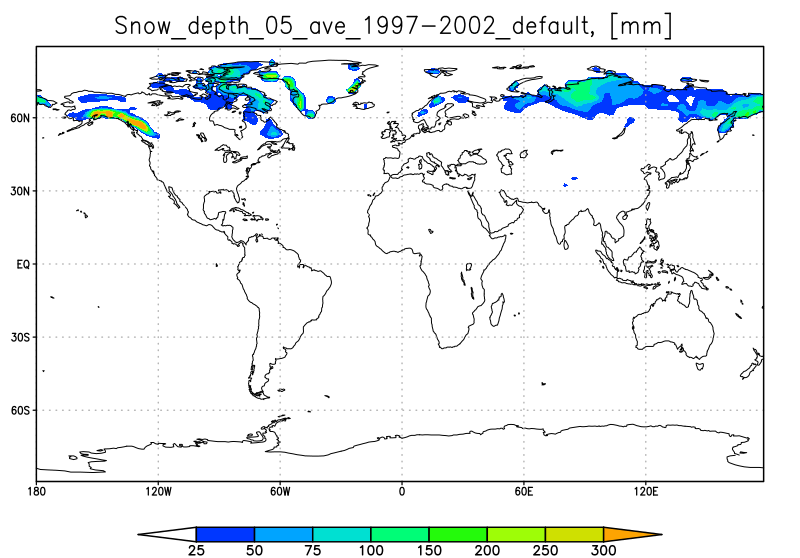
\includegraphics[width=1.1\linewidth]{pictures/Snow_depth_05_ave_1997-2002_default.png} \\ (а)}
    \end{minipage}
    \hfill
    \begin{minipage}{0.49\linewidth}
        \center{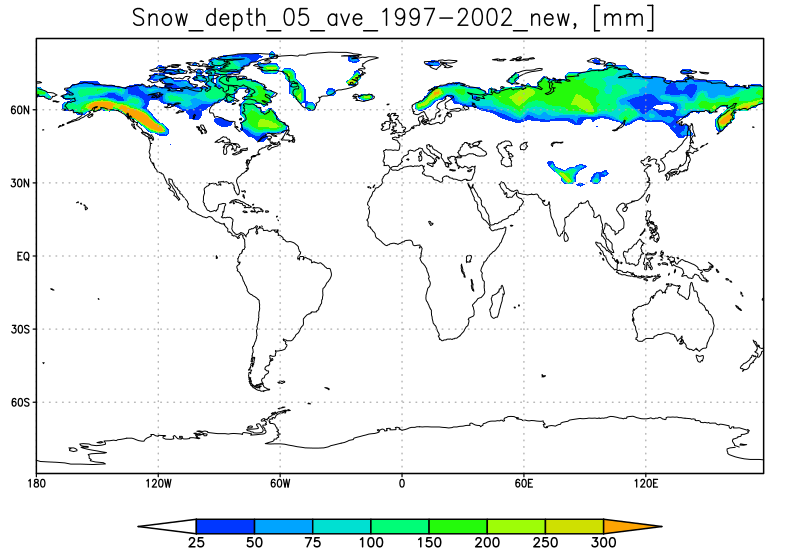
\includegraphics[width=1.1\linewidth]{pictures/Snow_depth_05_ave_1997-2002_new.png} \\ (б)}
    \end{minipage}
\end{figure}

\center{Среднемесячная водно-эквивалентная толщина слоя снега по данным (а) исходной и (б) модифицированной версий модели ИВМ (месяц -- май)}

\end{frame}



\begin{frame}{Результаты}

\scriptsize
\begin{figure}[h]
    \begin{minipage}[h]{0.48\linewidth}
        \center{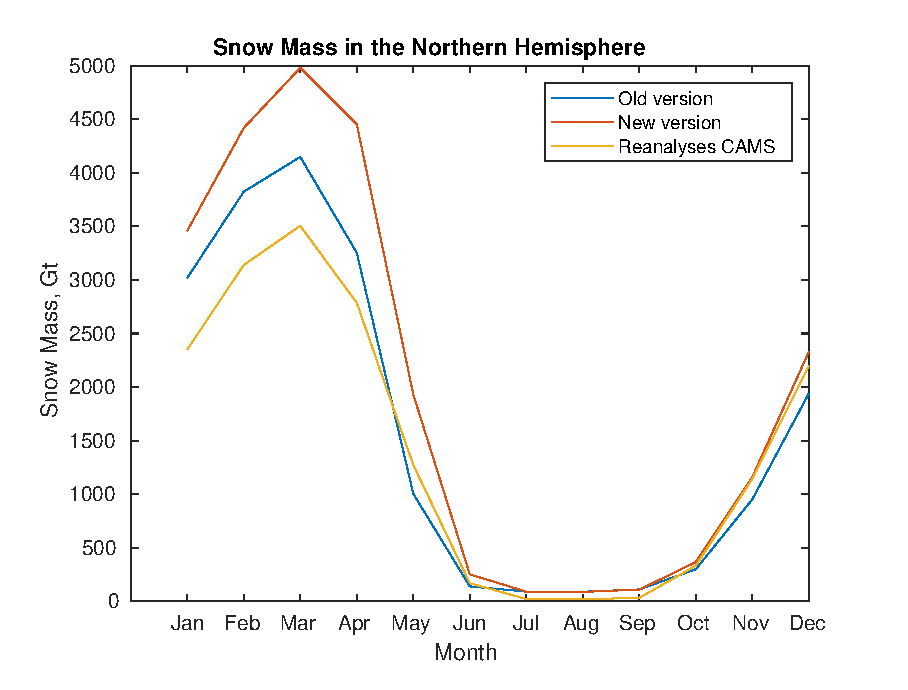
\includegraphics[width=1.1\linewidth]{SnowMass.eps} \\ (а) }
    \end{minipage}
    \hfill
    \begin{minipage}[h]{0.51\linewidth}
        \center{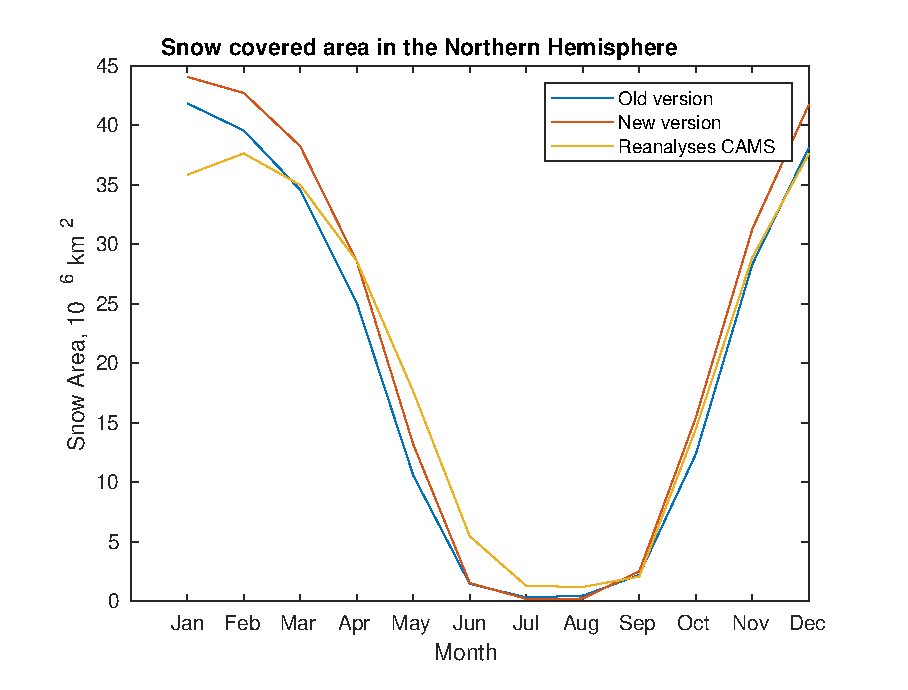
\includegraphics[width=1.1\linewidth]{SnowArea.eps} \\ (б) }
    \end{minipage}
\end{figure}
\center{Годовой ход (а) массы снега и (б) площади, покрытой им, осредненные за 1997-2002 годы по данным исходной и модифицированной версий модели, и по данным реанализа CAMS}

\end{frame}



\begin{frame}{Заключение}


\end{frame}



\begin{frame}{}
\begin{center}
    \Large{Спасибо за внимание!}
\end{center}
\end{frame}






\end{document}